\section{Cross-Validation}
\textbf{Problem with 80/20 Data Separation}
\begin{itemize}
    \item Test Error depends on random set
    \item For different Set, the test error would be different
\end{itemize}
\textbf{With Cross-Validation we can obtain a better estimate of the generalization error}

\columnbreak
\subsection{k-fold Cross-Validation}
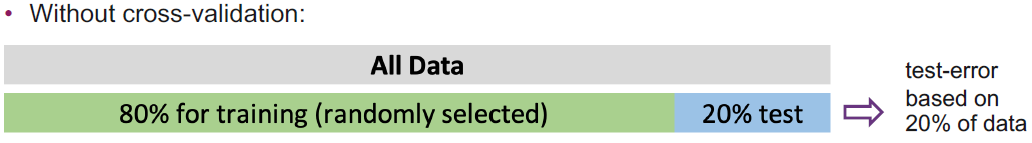
\includegraphics[width=\linewidth]{k_fold.png}
\textbf{With k-Fold Cross-Validation}\\
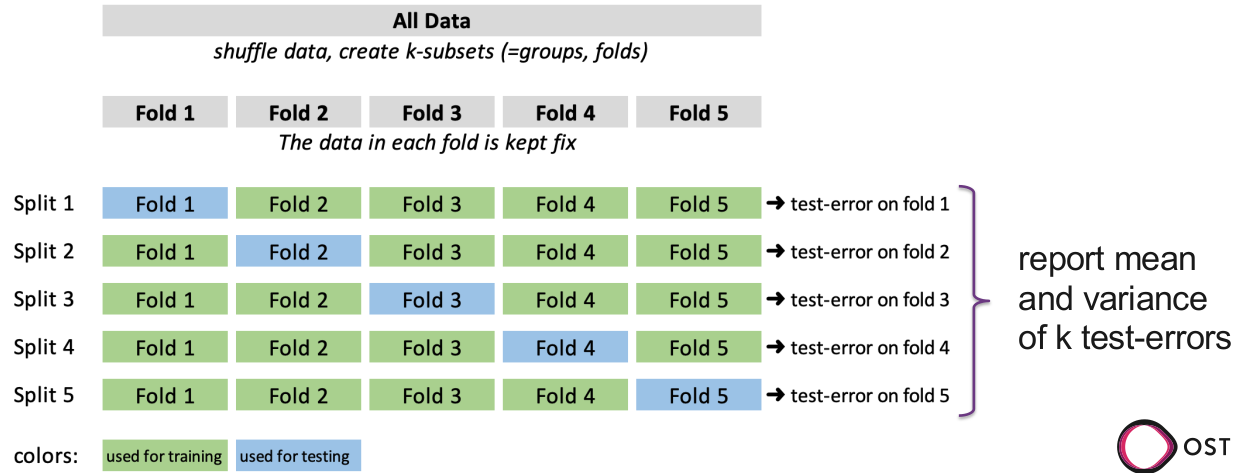
\includegraphics[width=\linewidth]{k_fold2.png}

\subsubsection{Some Comments}
\begin{itemize}
    \item Typical Values for k are 5,10 or N
    \item The data of a fold does not change during procedure
    \item Do not preprocess the whole dataset
    \item Apply the preprocessing pipe-line to each split
\end{itemize}

\section{Artificial Neural Networks (ANN)}
\subsection{Artificial Neurons}
\begin{itemize}
    \item Receives an input vector $[x_1,x_2, ...]$
    \item Each neuron has its own input weights $[w_1, w_2, ...]$ and \textbf{bias} b
    \item Calculates the sum of the weighted input (dot product $\vec{x} * \vec{w}$), adds a bias b, and passes it through a nonlinear activiation function
\end{itemize}
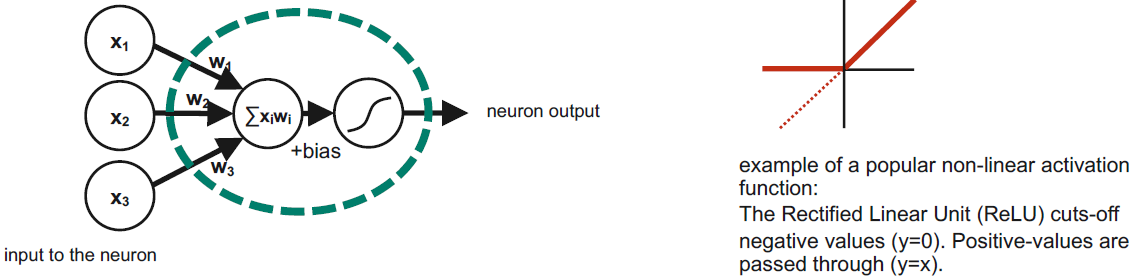
\includegraphics[width=\linewidth]{artificial_neurons.png}

\subsection{Simple ANN}
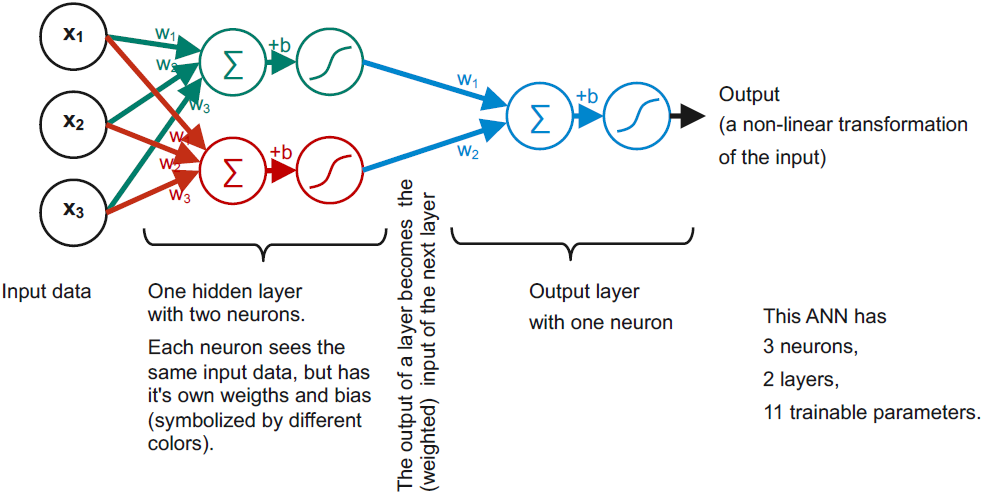
\includegraphics[width=\linewidth]{ann.png}

\subsection{Traning an ANN}
\textbf{Supervised learning}
\begin{itemize}
    \item Data with label
    \item For each input $\vec{x}$ we are given the output $\vec{y}$
    \item ANN is initialized with random weights
    \item An optimizer reduces a cost-function (e.g. MSE)
    \item At every iteration, and for every single weight $w$ and bias $b$, the partial derivative needs to be calculated. (Backpropagation)
\end{itemize}
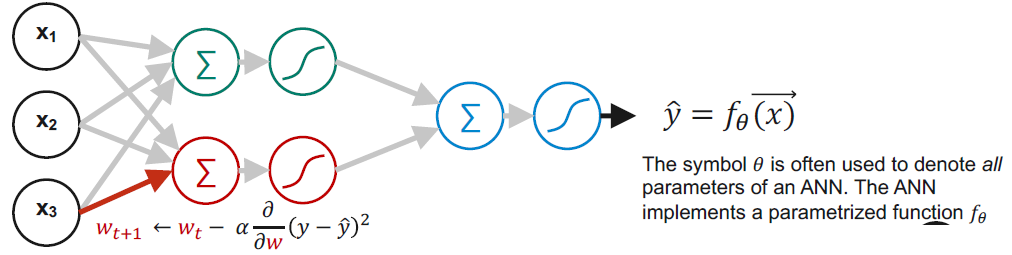
\includegraphics[width=\linewidth]{train_ann.png}
